\chapter{Fizikai modell}\label{chap:physical_system}

Ebben a fejezetben a robotujj egyszerűsített, egy szabadságfokú fizikai modellje kerül 
bevezetésre. A kapott dinamikai leírás lehetővé teszi az időkéséssel kiegészített 
stabilitásvizsgálatot. 

\section{Egyenáramú motor dinamikája}

\begin{figure}[b!]
\begin{center}
%\phantomsection{}
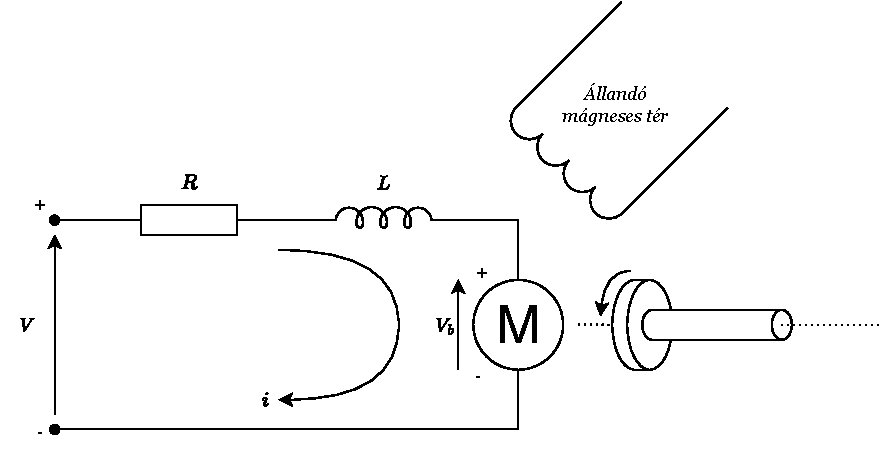
\includegraphics[width=\textwidth]{images/motor_model_electric.pdf}
\caption{Az egyenáramú motor áramköri diagramja}
\label{fig:dc_motor_electric}
\end{center}
\end{figure}

A robot motorjának modelljét a~\ref{fig:dc_motor_electric}. ábra szemlélteti. 
A felhasznált motor feltételezetten állandó gerjesztésű. Kifejtett nyomatéka a 
Biot--Savart-törvény szerint arányos a forgórészen átfolyó árammal. A forgórészben
indukált feszültség pedig arányos annak szögsebességével. 

A Lenz-törvény alapján 
\begin{equation}\label{eq:lenz_torque}
\begin{split}
    \tau_\RM m &= K_\RM \tau i, \\
    V_\RM b &= K_\RM e \dot\theta,
\end{split}
\end{equation}
ahol $K_\RM \tau$ a nyomatékállandó, $K_\RM e$ a sebesség-feszültség állandó, $\tau_\RM m$ a kifejtett 
nyomaték, $i$ a rotor árama, $V_\RM b$ a rotorban indukált feszültség és $\dot\theta$ a rotor szögsebessége.

Az energiamegmaradás törvénye alapján a két konstans értéke SI mértékegységben kifejezve megegyezik:
\begin{align}
    K_\RM m \stackrel{\text{def}}{=} K_\RM \tau = K_\RM e,
\end{align}
így a következőkben $K_\RM m$ paraméterként jelennek meg. 

A forgórész áramkörére Kirchhoff I. törvénye alapján felírható
\begin{align}\label{eq:armature_circuit}
    V - Ri - L\DIFF{i}{t} - K_\RM m\dot\theta = 0,
\end{align}
ahol $R$ a forgórész tekercsének ellenállása, $L$ a tekercs induktivitása, 
$K_\RM m$ a motorállandó, $V$ a motor feszültsége, $i$ a motoráram és $\theta$ a szögelfordulás.


A forgórészt merev testnek tekintve, annak mozgásegyenlete a dinamika alaptétele és a~\ref{fig:dc_motor_mechanical}. számú 
szabadtest-ábra alapján a következő alakban írható fel:
\begin{align}\label{eq:rotor_dynamics}
    J\ddot\theta + B_\RM m\dot\theta = \tau_\RM m + \tau_\RM e,
\end{align}
ahol $J$ a forgórész tehetetlensége, $B_\RM m$ a viszkózus csillapítási együttható, 
$K_\RM m$ a motorállandó, $\theta$ a szögelfordulás, $i$ a motoráram, $\tau_\RM m$ a motor által kifejtett nyomaték 
és $\tau_\RM e$ a forgórészre ható külső nyomaték. 
%
A~\eqref{eq:armature_circuit} és~\eqref{eq:rotor_dynamics} egyenletek egyértelműen leírják a 
rendszer időtartománybeli viselkedését.

\begin{figure}[t!]
	\begin{center}
		%\phantomsection{}
		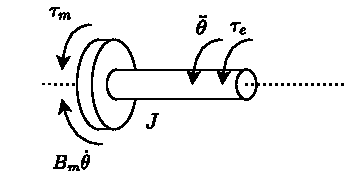
\includegraphics[width=9cm]{images/motor_model_mechanical.pdf}
		\caption{Az egyenáramú motor szabadtest ábrája}
		\label{fig:dc_motor_mechanical}
	\end{center}
\end{figure}

A további vizsgálathoz kedvezőbb a differenciálegyenleteket állapottér modellként felírni.
Az állapottér modell általánosan~\citep{kalman1963mathematical}
\begin{equation}\label{eq:state_space_generic}
\begin{split}
    \dot{\BF x} &= \BF A \BF x + \BF B \BF u\,,\\
    \BF y &= \BF C \BF x + \BF D \BF u
\end{split}
\end{equation} 
alakban írható fel. Legyen 
\begin{equation}
	\BF x := [\theta~~\dot \theta~~i]^{\mathsf T}
\end{equation}
az állapotvektor, emellett
\begin{equation}\label{eq:uinput27}
	\BF u := [\tau_\RM e~~V]^{\mathsf T}
\end{equation} 
a bemeneti vektor és \(y := \theta\) a kimenet.

A~\eqref{eq:armature_circuit} és a~\eqref{eq:rotor_dynamics} egyenleteket átrendezve 
az  \(\BF A\) rendszermátrix, a \(\BF B\) irányító mátrix, a \(\BF C\) megfigyelő mátrix és a \(\BF D\) előrecsatoló mátrix
\begin{equation}\label{eq:state_space}
    \begin{split}
        \BF A &= 
        \begin{bmatrix}
            0 & 1 & 0 \\
            0 & -\frac{B_\RM m}{J} & \frac{K_\RM m}{J} \\
            0 & -\frac{K_\RM m}{L} & -\frac{R}{L} \\
        \end{bmatrix}\,,\\
        \BF B &=
        \begin{bmatrix}
            0 & 0 \\
            1 & 0 \\
            0 & 1 \\
        \end{bmatrix}\,,\\
        \BF C &=
        \begin{bmatrix}
            1 & 0 & 0 \\
        \end{bmatrix}\,,\\
        \BF D &= \BF 0
    \end{split}
\end{equation}
alakban származtatható. 

A későbbiekben ismertetett kísérleti összeállítás paraméterei 
nem teszik lehetővé a forgórész áramának modellezését, ehhez bővebb indoklás az \ref{chap:experiment}.\,fejezetben található. 
%
Az induktivitással kiegészített modell mellett mindig megjelenik az 
induktivitás nélküli modell, ahol szükséges. 
%
Az egyszerűsített állapottér modell állapotvektora 
\(\BF x = [\theta~~\dot \theta]^{\mathsf T}\), az \(\BF u\) bemeneti vektora változatlan (lásd \eqref{eq:uinput27}), 
\(\BF A\), \(\BF B\), \(\BF C\) és \(\BF D\) mátrixa pedig 
%
\begin{equation}\label{eq:state_space_reduced}
    \begin{split}
        \BF A &= 
        \begin{bmatrix}
            0 & 1 \\
            0 & -\frac{B_\RM m R + K^2_\RM m}{JR} \\
        \end{bmatrix}\,,\\
        \BF B &=
        \begin{bmatrix}
            0 & 0 \\
            \frac{1}{J} & \frac{K_\RM m}{JR} \\
        \end{bmatrix}\,,\\
        \BF C &=
        \begin{bmatrix}
            1 & 0 \\
        \end{bmatrix}\,,\\
        \BF D &= \BF 0\,.
    \end{split}
\end{equation}

Az állapottér modellt felhasználva a frekvenciatartománybeli vizsgálatokhoz felírhatóak a rendszer 
szög-nyomaték és szög-feszültség átviteli függvényei, ezek általános alakja az alábbi:
\begin{align}\label{eq:transfer_generic}
    \frac{Y(s)}{U(s)} = \BF C{\left(s \BF I - \BF A\right)}^{-1} \BF B\,,
\end{align}
ahol $\BF I$ az identitás mátrix.

Behelyettesítve~\eqref{eq:state_space} 
paramétereit~\eqref{eq:transfer_generic} alapján a karakterisztikus polinom a
\begin{align}\label{eq:characteristic_polynomial}
    p(s) = s\left(JLs^2 + \left(B_\RM m L + JR\right)s + K_\RM m^2 + B_\RM m R\right)
\end{align}
alakban adódik. Az átviteli függvények pedig ez alapján
\begin{equation}\label{eq:transfer_function}
    \begin{split}
        \frac{\theta(s)}{\tau_\RM e(s)} &= \frac{Ls + R}{p(s)}\,,\\
        \frac{\theta(s)}{V(s)} &= \frac{K_\RM m}{p(s)}\,.
    \end{split}
\end{equation}

Az induktivitás elhanyagolása esetén az előzőekhez hasonlóan származtatható a karakterisztikus polinom:
\begin{align}\label{eq:characteristic_polynomial}
    p(s) = s\left(JRs + K_\RM m^2 + B_\RM m R\right),
\end{align}
valamint az átviteli függvények szintén egyszerűsödnek:
\begin{equation}\label{eq:transfer_function}
    \begin{split}
        \frac{\theta(s)}{\tau_\RM e(s)} &= \frac{R}{p(s)}\,,\\
        \frac{\theta(s)}{V(s)} &= \frac{K_\RM m}{p(s)}.
    \end{split}
\end{equation}

\section{Egyenáramú motor stabilitása}
A motormodell stabilitási tulajdonságai a~\eqref{eq:characteristic_polynomial} egyenletben szereplő karakterisztikus 
polinom segítségével meghatározhatók.
A karakterisztikus polinom egyik zérusa az origóban helyezkedik el. Ebből következik, hogy a rendszer
egységugrás bemenetre korlátlanul nagy szögelfordulással válaszol. Ez utóbbi a jelen alkalmazásban nem elfogadható. 
Ha a szabályozókör visszacsatoló ága megszakad, a motor a megengedhető mozgástartományon kívülre fordulhat.
A biztonságos működéshez szükséges például egy végálláskacsolót beépíteni, mely segítségével a motor 
mozgása a szabályozástól függetlenül is az előírt tartományon belülre korlátozható.

\section{Megfigyelhetőség}\label{chap:observability}
A felhasznált szenzorok számának minimalizálása érdekében a lehető legkevesebb belső állapot közvetlen mérése 
a cél. A továbbiakban egyedül a szögelfordulás áll elő közvetlen mérésből. 
A szabályozó teljes állapotvisszacsatolásra épül, így a kimenet mérésével minden további belső állapot 
megfigyelhető kell legyen. 
A~\eqref{eq:state_space_generic} és~\eqref{eq:state_space} egyenletek alapján a kimeneti megfigyelhetőség feltétele, hogy a
\begin{align}\label{eq:observability_generic}
    \left[\begin{array}{c}
        \BF{C} \\ \hline
        \BF{CA} \\ \hline
        \BF C \BF A^2
    \end{array}\right]
\end{align}
mátrix legyen maximális rangú. A feltételben szereplő mátrixot a motorparaméterekkel kifejezve 
a~\eqref{eq:state_space} egyenlet alapján:
\begin{align}
    \begin{bmatrix}
        1 & 0 & 0 \\
        0 & 1 & 0 \\
        0 & -\frac{B_\RM m}{J} & \frac{K_\RM m}{J}
    \end{bmatrix},
\end{align}
mely redukált lépcsős alakra hozható:
\begin{align}
    \begin{bmatrix}
        1 & 0 & 0 \\
        0 & 1 & 0 \\
        0 & 0 & 1
    \end{bmatrix}.
\end{align}
Ez valóban maximális rangú, tehát a rendszer minden állapota megfigyelhető a szögelfordulás méréséből.

Az induktivitást elhanyagolva a megfigyelhetőség feltétele
még egyszerűbb alakkal rendelkezik, a megfigyelhetőségi mátrix ekkor:
\begin{align}
	\left[\begin{array}{c}
		\BF{C} \\ \hline
		\BF{CA} \\
	\end{array}\right].
\end{align}
Behelyettesítve az egyszerűsített modell \eqref{eq:state_space_reduced} paramétereit ez a megfigyelhetőségi mátrix azonnal redukált lépcsős alakban adódik:
\begin{align}
    \begin{bmatrix}
        1 & 0 \\
        0 & 1 \\
    \end{bmatrix}.
\end{align}
Ezáltal a rendszer minden állapota megfigyelhető ebben az esetben is. 


\clearpage


\section{Irányíthatóság}\label{chap:controllability}
A szabályozó akkor tudja követni a számára előírt impedanciamodellt, 
ha megfelelő bemeneti feszültség alkalmazásával eljuttatható az előírt állapotba~\citep{kalman1963controllability}.

A rendszer pólusai áthelyezhetők kell legyenek az impedanciamodell pólusaiba, 
ehhez pedig a rendszer teljesen állapot irányítható kell legyen.
A~\eqref{eq:state_space_generic} egyenlet állapottér modellje alapján a teljes állapot irányíthatóság feltétele, hogy a
\begin{align}\label{eq:controllability_generic}
    \left[\begin{array}{c|c|c}
        \BF{B}_\RM V & \BF{A} \BF{B}_\RM V & \BF A^2 \BF{B}_\RM V
    \end{array}\right]
\end{align}
irányíthatósági mátrix maximális rangú legyen. \(\BF{B}_\RM V\) az irányító mátrix azon része, mely a 
feszültségjel állapotra gyakorolt hatását tartalmazza. 
Felhasználva a~\eqref{eq:state_space} kifejezés paramétereit a~\eqref{eq:controllability_generic} feltételben szereplő mátrix
\begin{align}
    \begin{bmatrix}
        0 & 0 & \frac{K_\RM m}{JL} \\
        0 & \frac{K_\RM m}{JL} & -\frac{K_\RM m\left(B_\RM m L + JR\right)}{J^2 L^2} \\
        \frac{1}{L} & -\frac{R}{L^2} & -\frac{K^2_\RM m L + JR^2}{J L^3} \\
    \end{bmatrix},
\end{align}
alakba írható át. Továbbá ez a mátrix redukált lépcsős alakban
\begin{align}
    \begin{bmatrix}
        1 & 0 & 0 \\
        0 & 1 & 0 \\
        0 & 0 & 1 \\
    \end{bmatrix},
\end{align}
mely mátrix rangja megegyezik sorainak számával, így az teljes állapot irányíthatóság feltétele teljesül.

Az induktivitást elhanyagolva az irányíthatósági feltételben megjelenő mátrix 
\begin{align}
    \left[\begin{array}{c|c}
        \BF{B} & \BF{AB}
    \end{array}\right].
\end{align}
Az egyszerűsített modell paramétereit behelyettesítve 
a
\begin{align}
    \begin{bmatrix}
        1 & 0 \\
        0 & 1 \\
    \end{bmatrix}
\end{align}
irányíthatósági mátrixot kapjuk.
Ez láthatóan megfelel a feltételnek, tehát az induktivitást elhanyagoló modell is teljes állapot irányítható.

